\documentclass{article}
\usepackage{graphicx}
\usepackage{wrapfig}
\usepackage{filecontents}
\usepackage{siunitx}
\usepackage[table]{xcolor}
\usepackage{float}
\usepackage{hyperref}

\usepackage{color} % balíček pro obarvování textů
\usepackage{xcolor}  % zapne možnost používání barev, mj. pro \definecolor
\usepackage{pgfplots} % http://www.chiark.greenend.org.uk/doc/texlive-doc/latex/pgfplots/pgfplots.pdf

\ifnum 0\ifxetex 1\fi\ifluatex 1\fi=0 % if pdftex
  \usepackage[T1]{fontenc}
  \usepackage[utf8]{inputenc}
\else % if luatex or xelatex
  \ifxetex
    \usepackage{mathspec}
  \else
    \usepackage{fontspec}
  \fi
  \defaultfontfeatures{Ligatures=TeX,Scale=MatchLowercase}
\fi
\usepackage[total={175mm,230mm}, top=23mm, left=20mm, includefoot]{geometry}
\hypersetup{
    colorlinks,
    linkcolor={blue!50!black},
    citecolor={green!50!black},
    urlcolor={blue!80!black}
}
\definecolor{orange}{RGB}{ 251, 114, 032}
\definecolor{fialova}{RGB}{ 255, 000, 255}

\newcounter{obrazky}
\setcounter{obrazky}{1}
\newcommand \obrlabel[1]
{ 
  obr.~\theobrazky
  \stepcounter{obrazky}
  \label{#1}
}


\newcommand \obr[1]
{ obr.~\ref{#1}}

\newcommand \tab[1]
{ tab.~\ref{#1}}


\begin{document}
\section{Nízkofrekvenční zesilovače s OZ}
\subsection*{Střídavý zesilovač s nesymetrickým napájením operačního zesilovače}
\begin{figure}[H]
  \begin{minipage}[t]{0.48\textwidth}
    \vspace{10mm}
    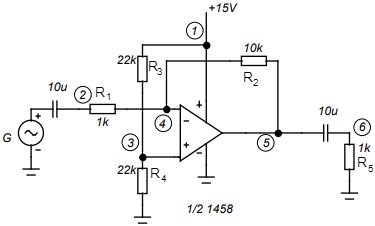
\includegraphics[width=\textwidth]{uvod/posun.png}
  \end{minipage}
  \hfill
  \begin{minipage}[t]{0.48\textwidth}
    % \vspace{-50mm}
    Abychom si vystačili s jedním zdrojem vytvoříme referenční napětí pro neinvertující vstup.

    \subsection{DC}
      Na vstupu je kondenzátor a do vstupu OZ neteče žádný proud \(\Rightarrow\) skrz \(R_1\) a \(R_2\) neteče žádný proud.
      V uzlech \(2, 4, 5\) a \(3\) je tedy stejné napětí a to \(U\frac{R_4}{R_4 + R_3} = \Left(15\frac{22\cdot10^{3}}{22\cdot10^{3}+22\cdot10^{3}} \Right) \-[V]= 7.5\-[V]\)
    \subsection{AC} 
      Na vstup přivedeme \(1\-[V]\) s frekvencí \(1\-[kHz]\)
      \(
        U_{5} = -\frac{R_2}{R_1} U_{vst} = -\frac{10\cdot10^{3}}{1\cdot10^{3}} \cdot 1 = -10\-[V]
      \)    
  \end{minipage}
\end{figure}

\subsection*{Sumační zesilovač}
\begin{figure}[H]
  \begin{minipage}[t]{0.48\textwidth}
    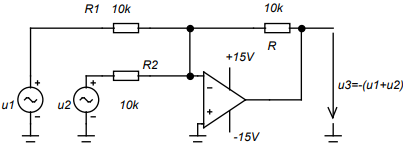
\includegraphics[width=\textwidth]{uvod/sou.png}
  \end{minipage}
  \hfill
  \begin{minipage}[t]{0.48\textwidth}
    \vspace{-20mm}
    \(
      U_{1} = 0\-[V] \Rightarrow I_{R1} = \frac{U_1}{R_1} ; I_{R1} = \frac{U_2}{R_2}

      I_{R3} = I_{R1} + I_{R2} \Rightarrow U_3 = R_3 I_{R3} = R_3\left(\frac{U_1}{R_1} + \frac{U_2}{R_2}\right) \\ U_3 = \frac{R_3}{R_1} U_1 + \frac{R_3}{R_2} U_2
    \)
  \end{minipage}
\end{figure}

\subsection*{Diferenční zesilovač}
\begin{figure}[H]
  \begin{minipage}[t]{0.48\textwidth}
    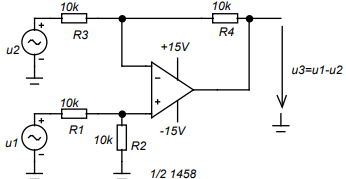
\includegraphics[width=\textwidth]{uvod/odc.png}
  \end{minipage}
  \hfill
  \begin{minipage}[t]{0.48\textwidth}
    \vspace{-35mm}
    \(
      U_{BA} = 0\-[V] \Rightarrow U_A = U_B = U_1 \frac{R_2}{R_2+R_1}

      I_{R3} = I_{R4} = \frac{U_2-U_A}{R_3} = \frac{U_2-U_1\frac{R_2}{R_2+R_1}}{R_3}

      U_3 = U_A - I_{R4}R_4 = U_1 \frac{R_2}{R_2+R_1} - \frac{U_2-U_1\frac{R_2}{R_2+R_1}}{R_3}R_4
    \)
  \end{minipage}
\end{figure}




\section*{Simulace}
\subsection*{Střídavý zesilovač s nesymetrickým napájením operačního zesilovače}
\begin{figure}[H]
  \begin{minipage}[t]{\textwidth}
    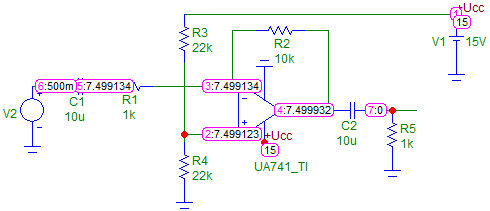
\includegraphics[width=\textwidth]{PC/ukol1/DC.png}
  \end{minipage}
\end{figure}

\begin{table}[H]
  \centering
  \begin{tabular}{|c|c|c|c|c|c|c|} 
    \hline
    uzel \(n\)          & 1       & 2      & 3     & 4     & 5       & 6      \\ \hline
    DC \(U_{nG}\-[V]\)  & 15.074  & 7.536  & 7.539 & 7.536 & 7.537   & 0      \\ \hline
    AC \(U_{nG}\-[mV]\) & 4.800   & 67.307 & 2.327 & 2.894 & 659.685 & 656.3  \\ \hline
  \end{tabular}
  \normalsize
  \caption{\label{tab_pracovni_bod_rozladeni1} Napětí v uzlech zaměřené na LC (čísla uzlu dle schematu v zadání)}
\end{table}

\begin{figure}[H]
  \begin{minipage}[t]{\textwidth}
    \centering
    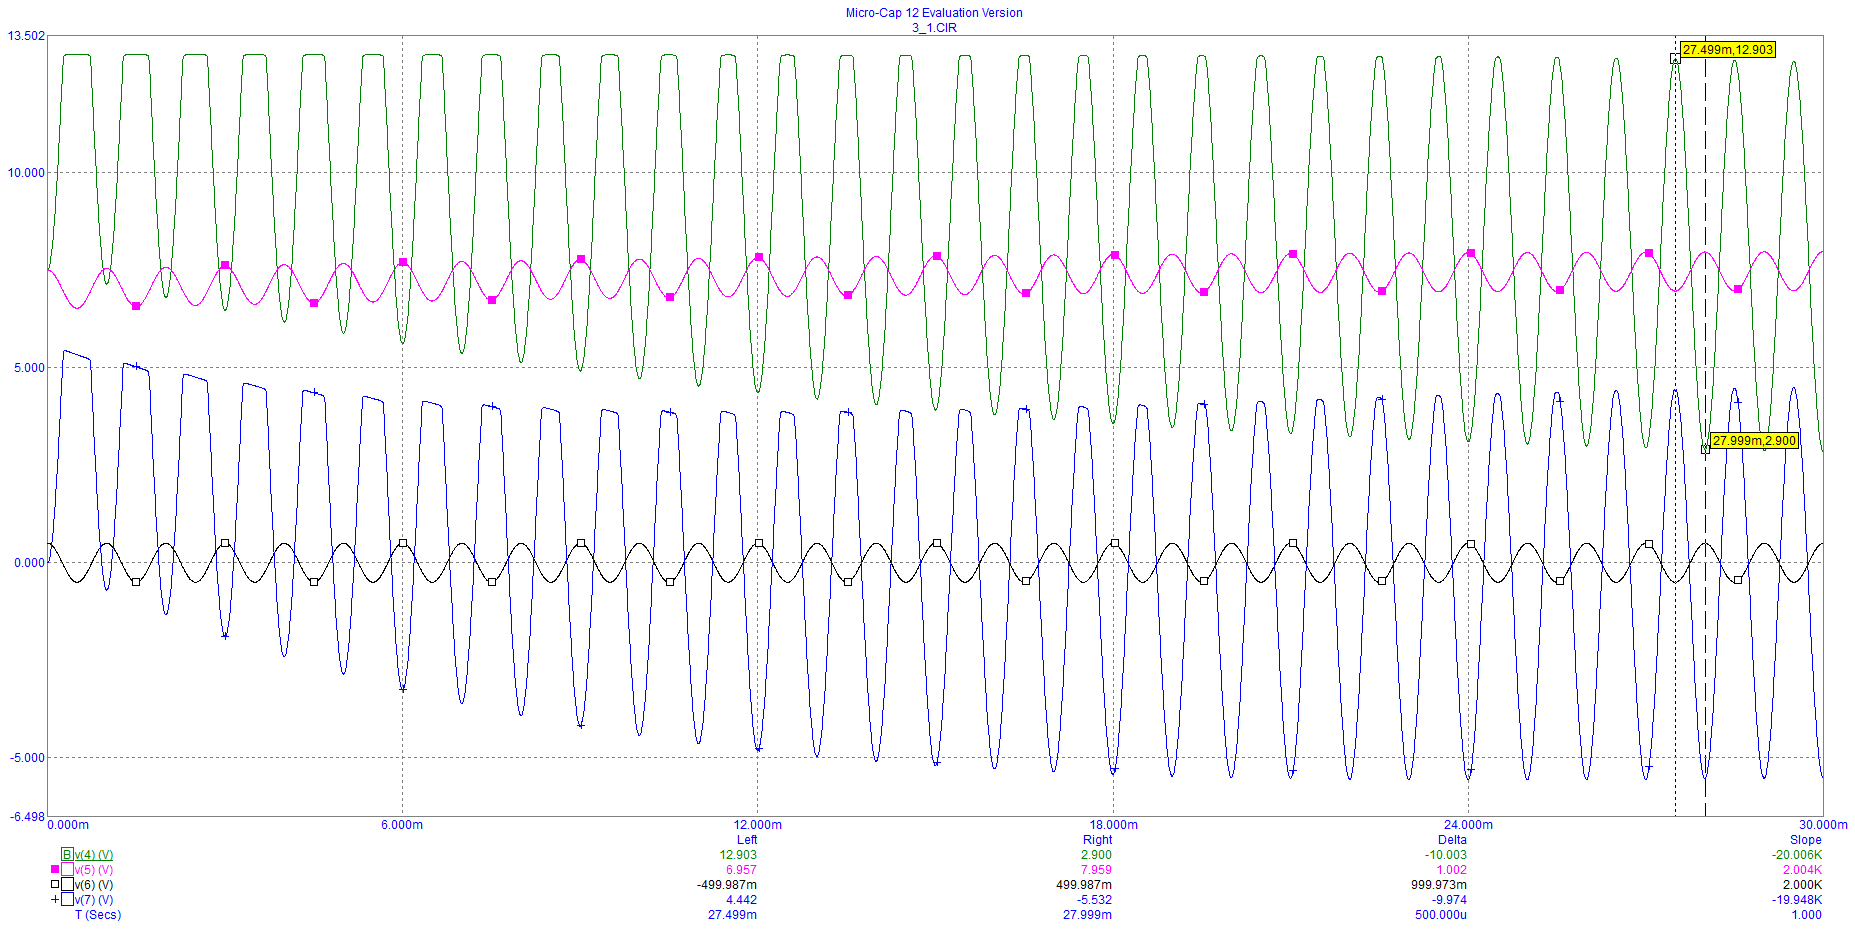
\includegraphics[width=\textwidth]{PC/ukol1/transient.png}
    Časový průběh s vyznačenými maximy na výstupu OZ.
  \end{minipage}
\end{figure}

\begin{figure}[H]
  \begin{minipage}[t]{\textwidth}
    \centering
    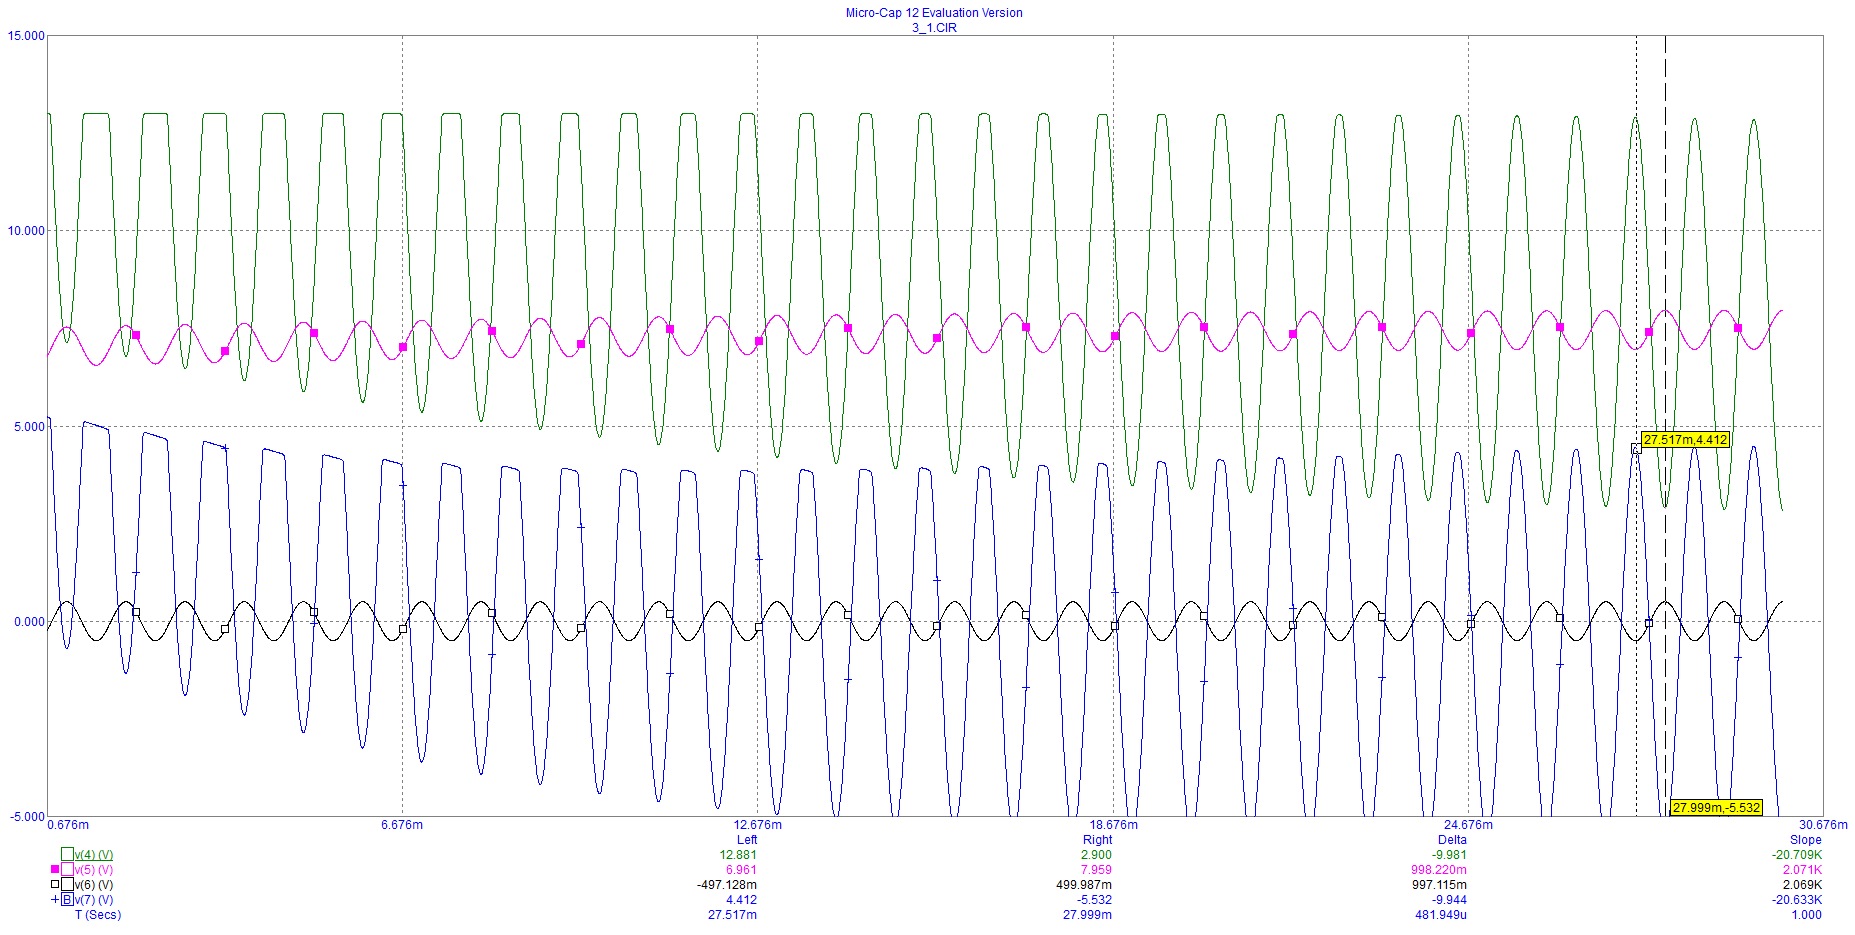
\includegraphics[width=\textwidth]{PC/ukol1/transient7.png}
    Časový průběh s vyznačenými maximy na výstupu zapojení.
  \end{minipage}
\end{figure}

\begin{figure}[H]
  \begin{minipage}[t]{\textwidth}
    \centering
    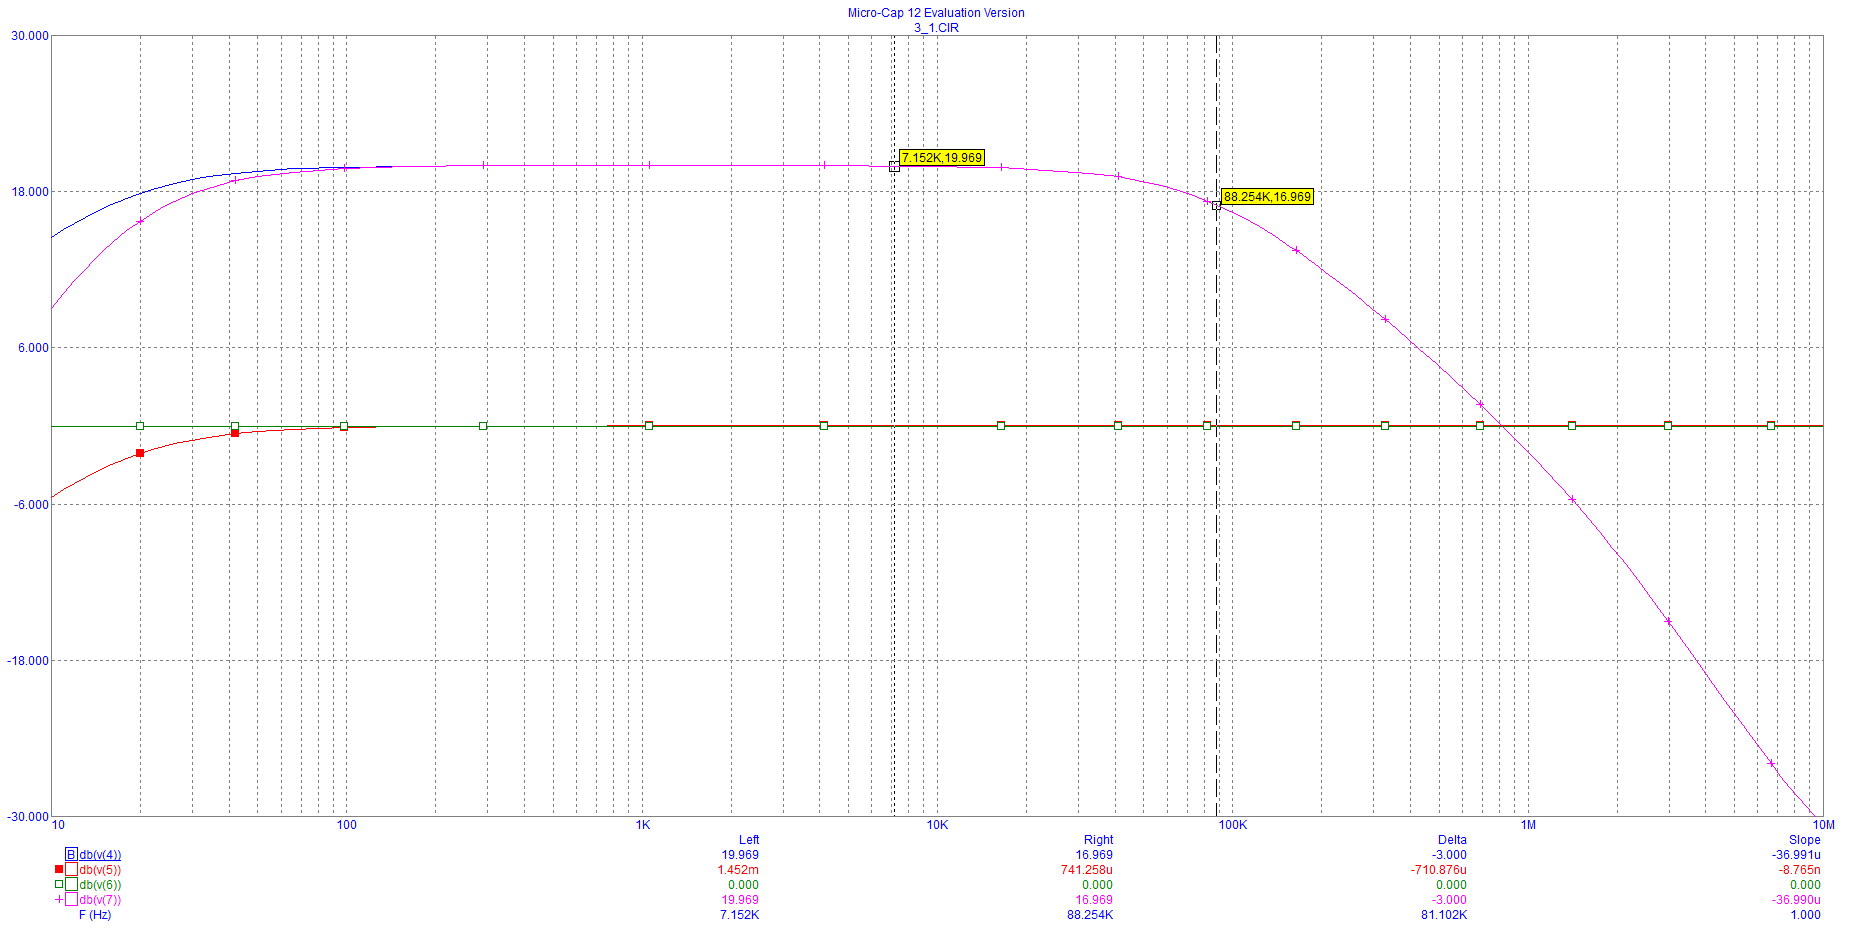
\includegraphics[width=\textwidth]{PC/ukol1/AC2.png}
    Amplitudová kmitočtová charakteristika
  \end{minipage}
\end{figure}

\begin{figure}[H]
  \begin{minipage}[t]{\textwidth}
    \centering
    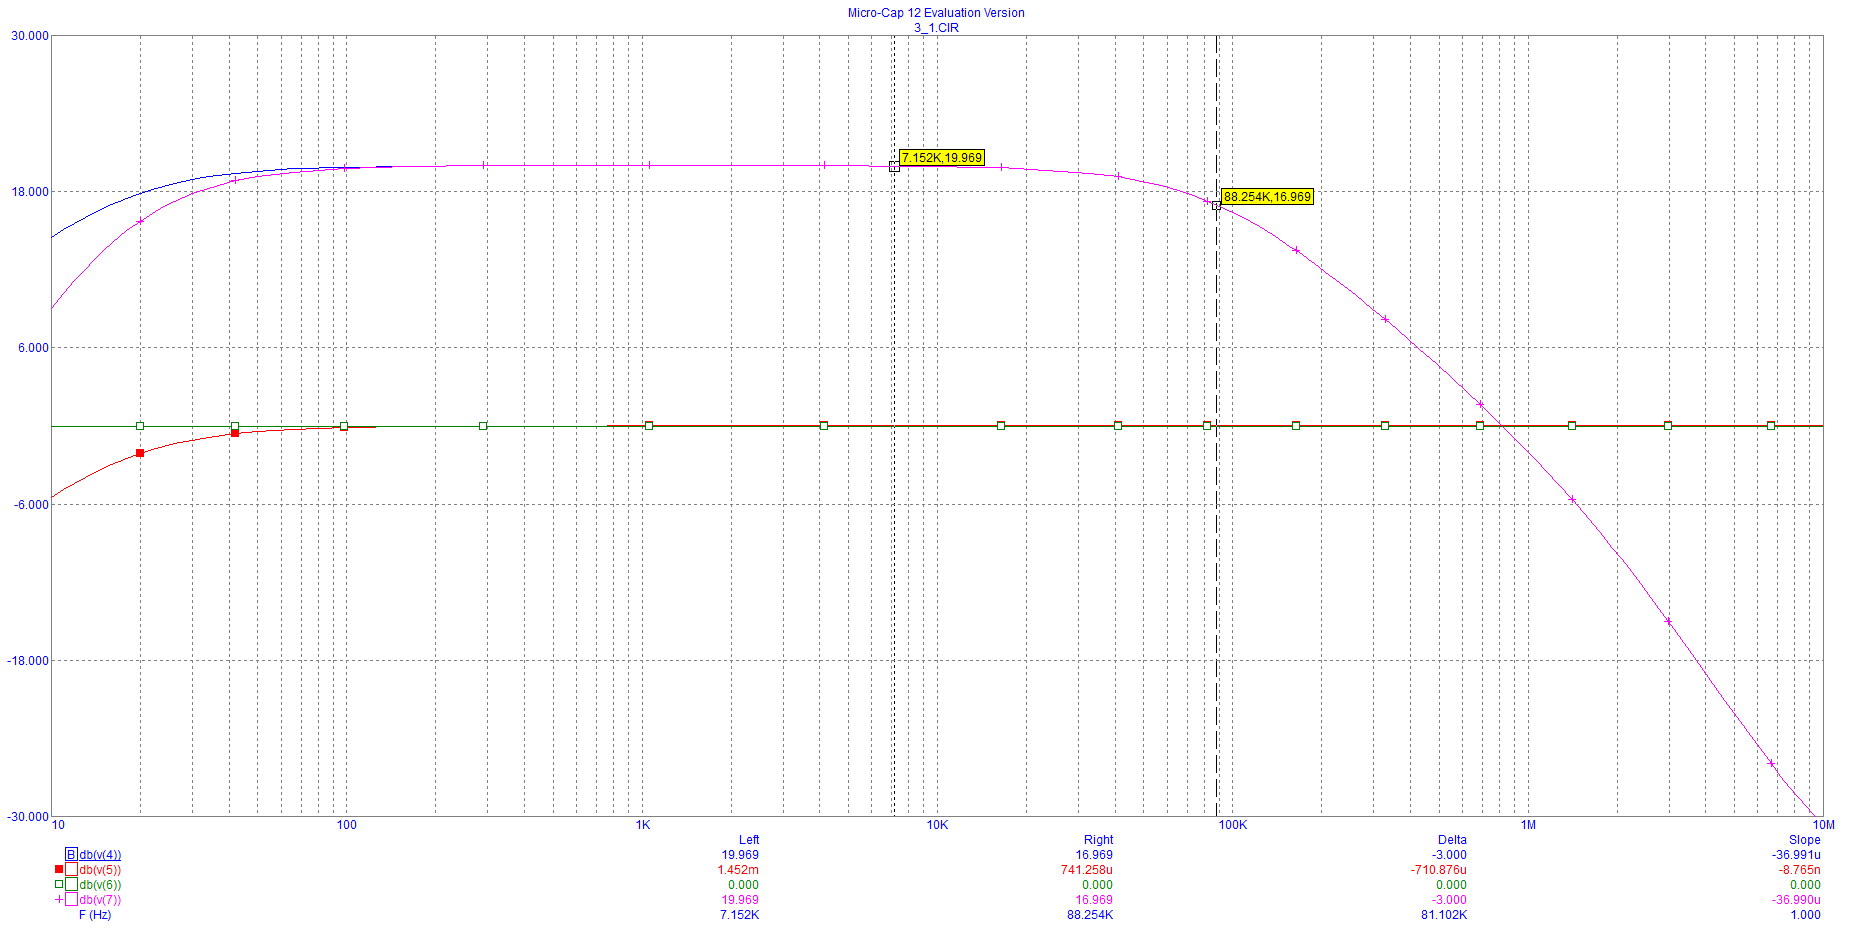
\includegraphics[width=\textwidth]{PC/ukol1/AC2.png}
    Amplitudová kmitočtová charakteristika
  \end{minipage}
\end{figure}

\subsection*{Sumační zesilovač}
\begin{figure}[H]
  \begin{minipage}[t]{\textwidth}
    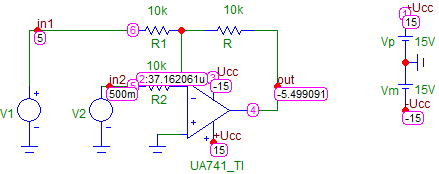
\includegraphics[width=\textwidth]{PC/ukol2/DC.png}
  \end{minipage}
\end{figure}

\begin{figure}[H]
  \begin{minipage}[t]{\textwidth}
    \centering
    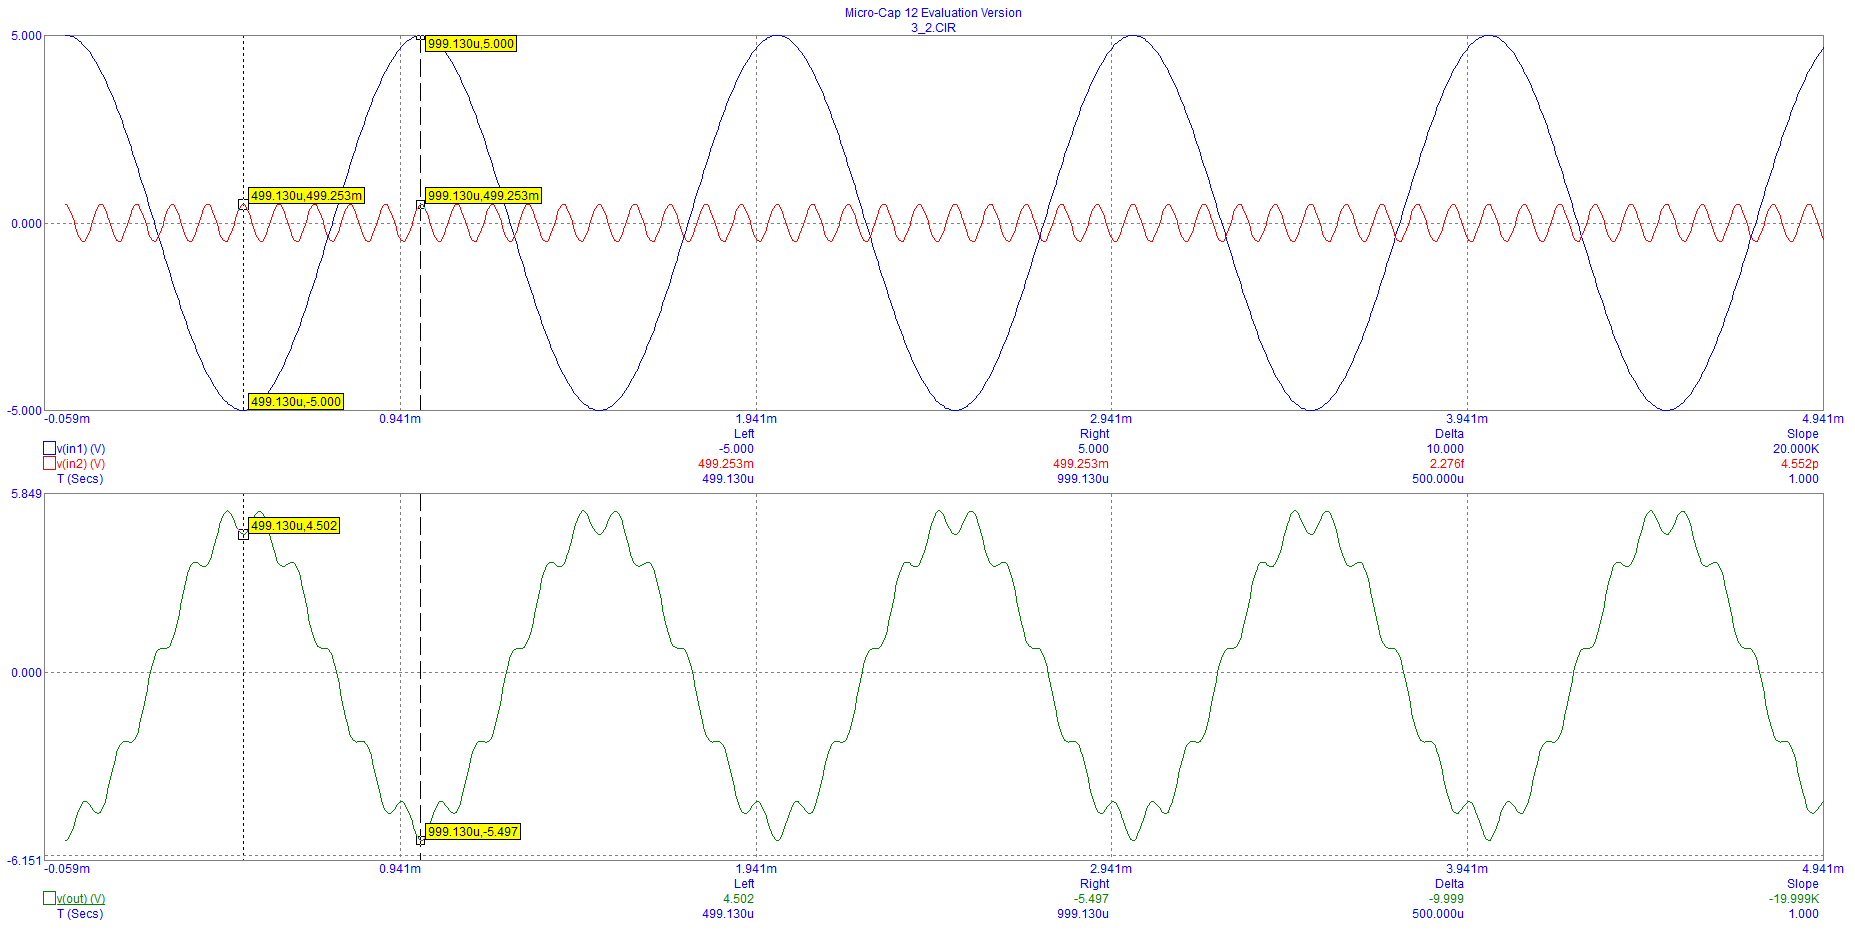
\includegraphics[width=\textwidth]{PC/ukol2/transient2.png}
    Časový průběh se dvěmy rozdílnými vstupními signály \\
    signál-1 \(U_{pp} = 10\-[V]\) \(f = 1\-[kHz]\) \\
    signál-2 \(U_{pp} = 1\-[V]\) \(f = 10\-[kHz]\).
  \end{minipage}
\end{figure}

\begin{figure}[H]
  \begin{minipage}[t]{\textwidth}
    \centering
    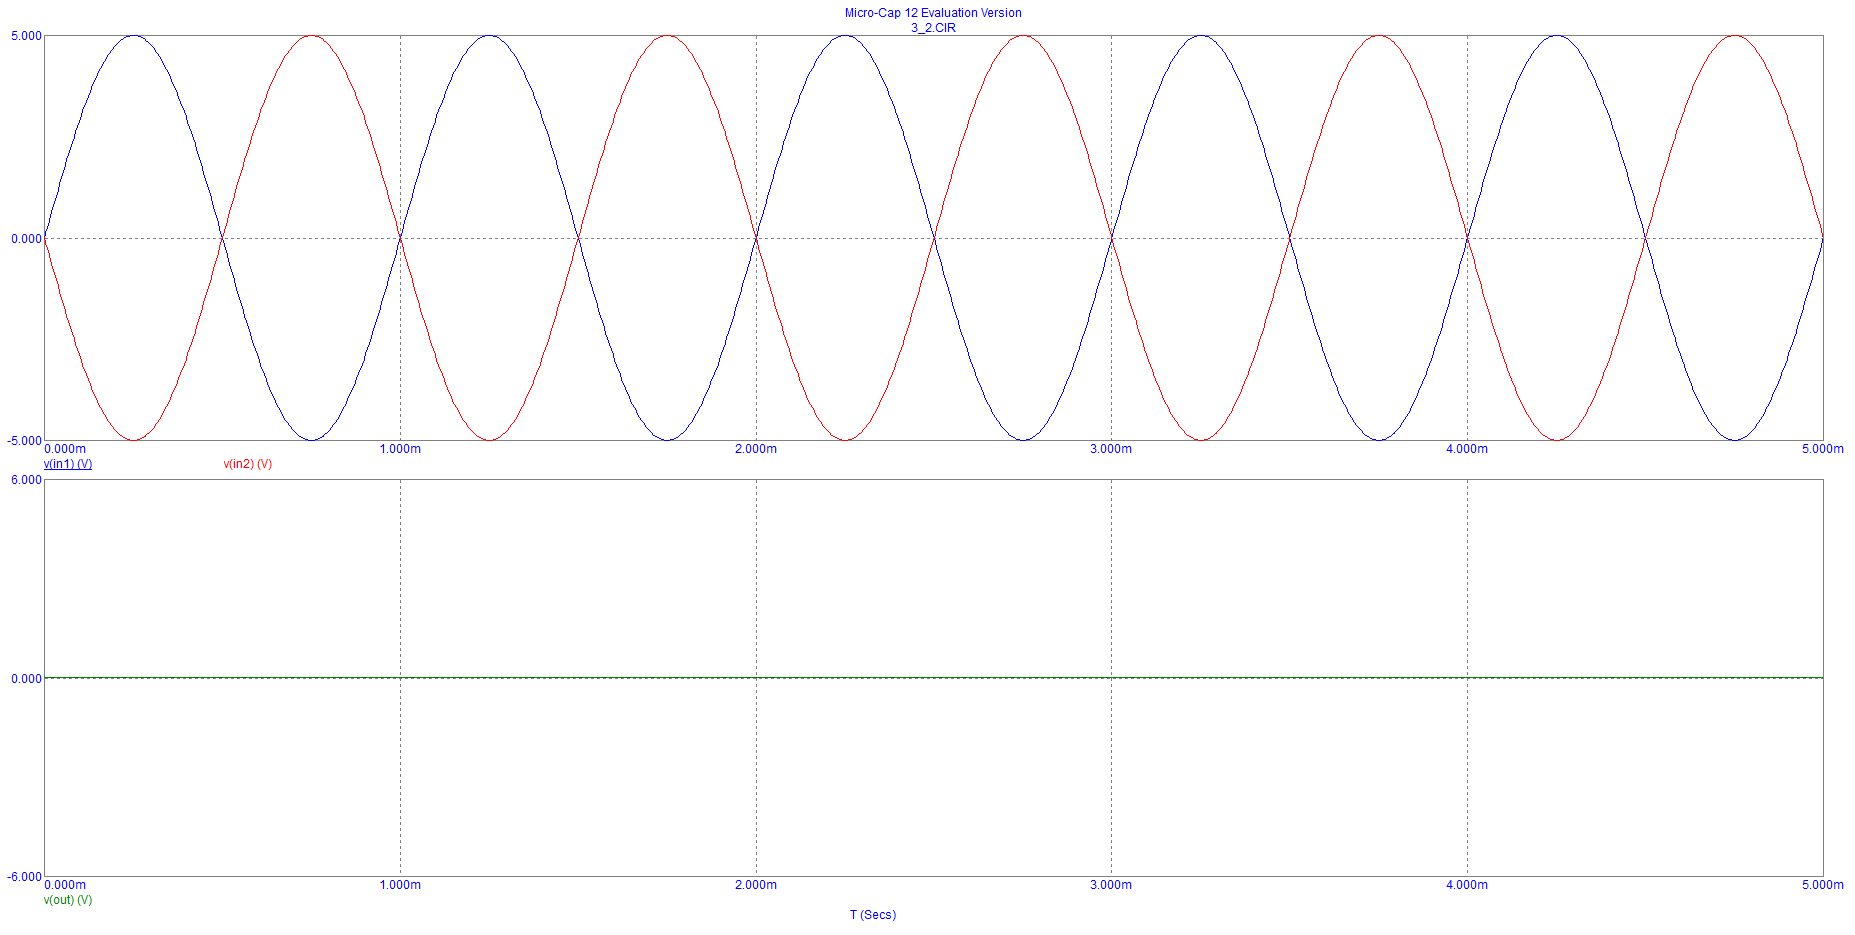
\includegraphics[width=\textwidth]{PC/ukol2/nula_vzstup.png}
    Časový průběh se dvěmy vstupními signály lišící se vzájemným posunutými \(180^\circ\) \(U_{pp} = 10\-[V]\) \(f = 1\-[kHz]\)
  \end{minipage}
\end{figure}

\subsection*{Diferenční zesilovač}
\begin{figure}[H]
  \begin{minipage}[t]{\textwidth}
    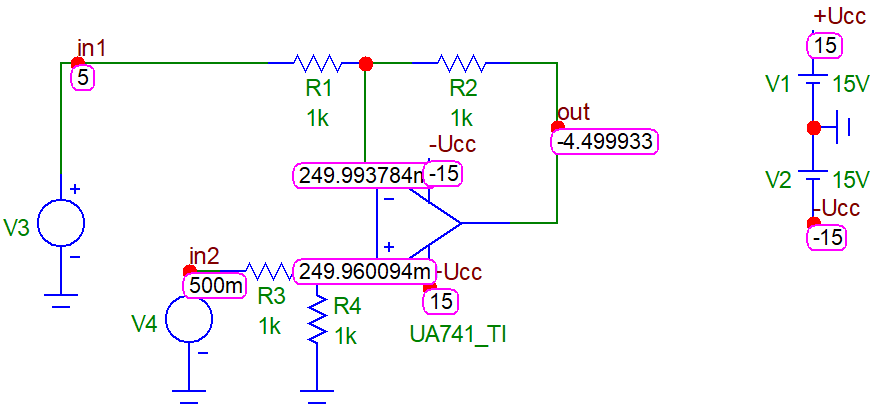
\includegraphics[width=\textwidth]{PC/ukol3/DC.png}
  \end{minipage}
\end{figure}

\begin{figure}[H]
  \begin{minipage}[t]{\textwidth}
    \centering
    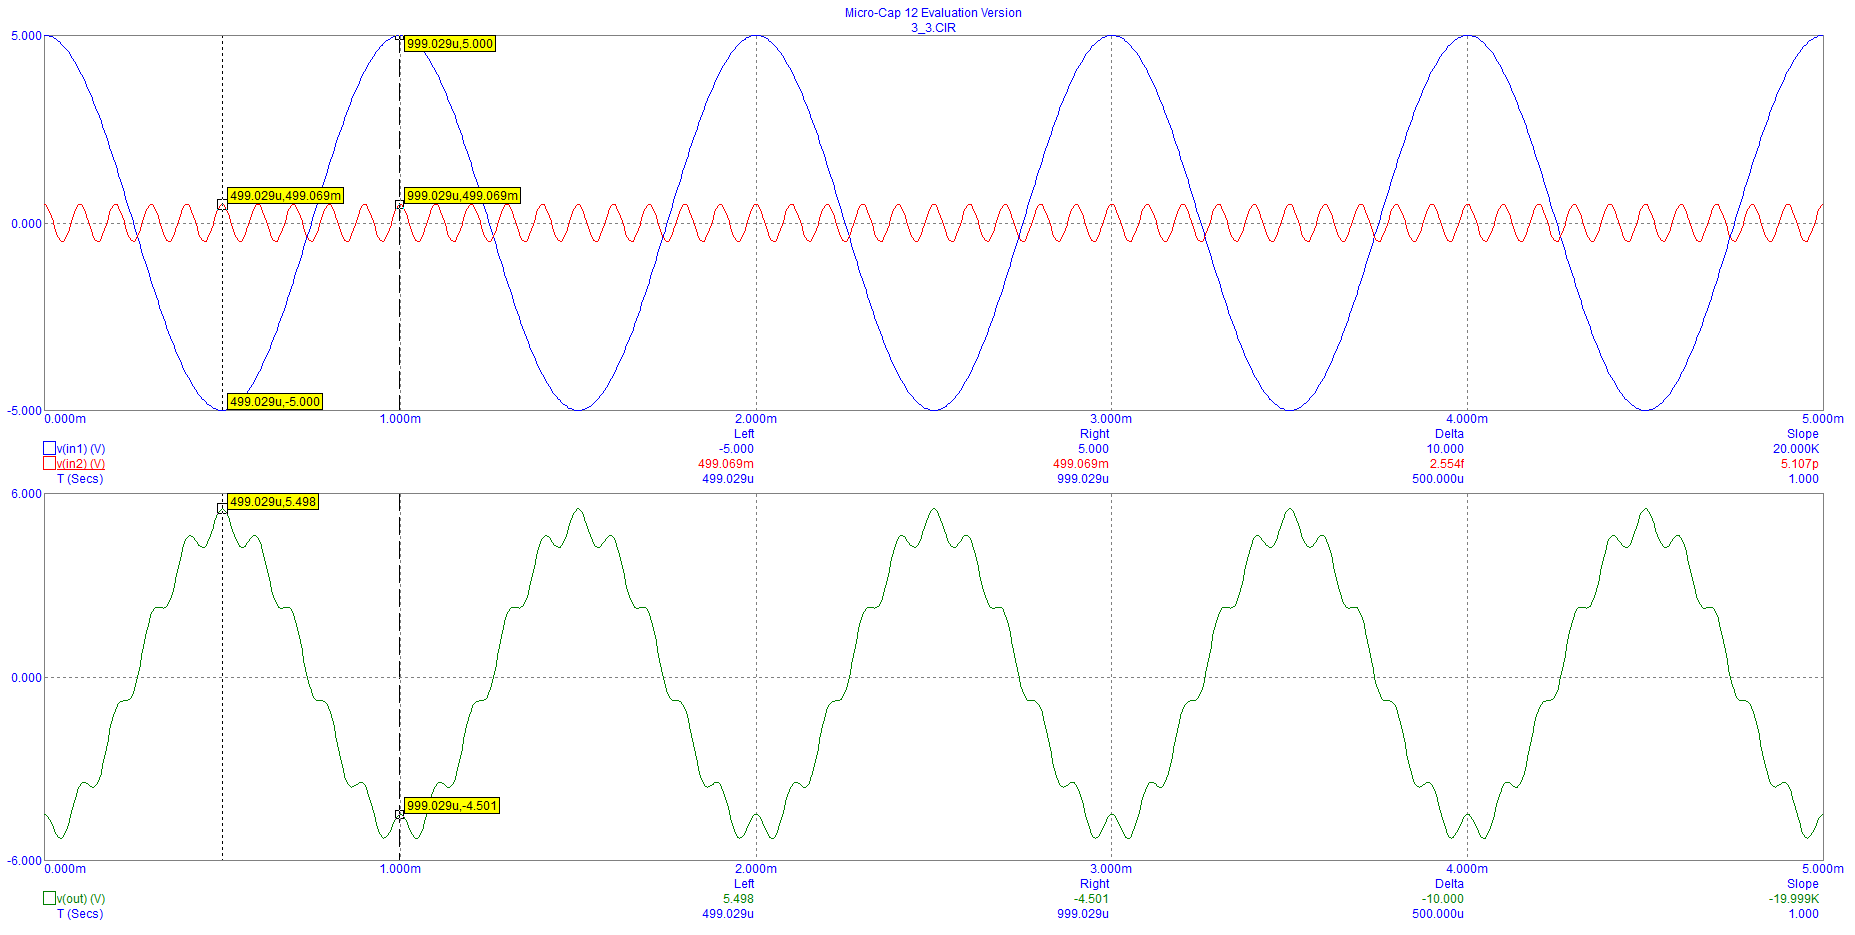
\includegraphics[width=\textwidth]{PC/ukol3/transient4.png}
    Časový průběh se dvěmy rozdílnými vstupními signály \\
    signál-1 \(U_{pp} = 10\-[V]\) \(f = 1\-[kHz]\) \\
    signál-2 \(U_{pp} = 1\-[V]\) \(f = 10\-[kHz]\).
  \end{minipage}
\end{figure}

\begin{figure}[H]
  \begin{minipage}[t]{\textwidth}
    \centering
    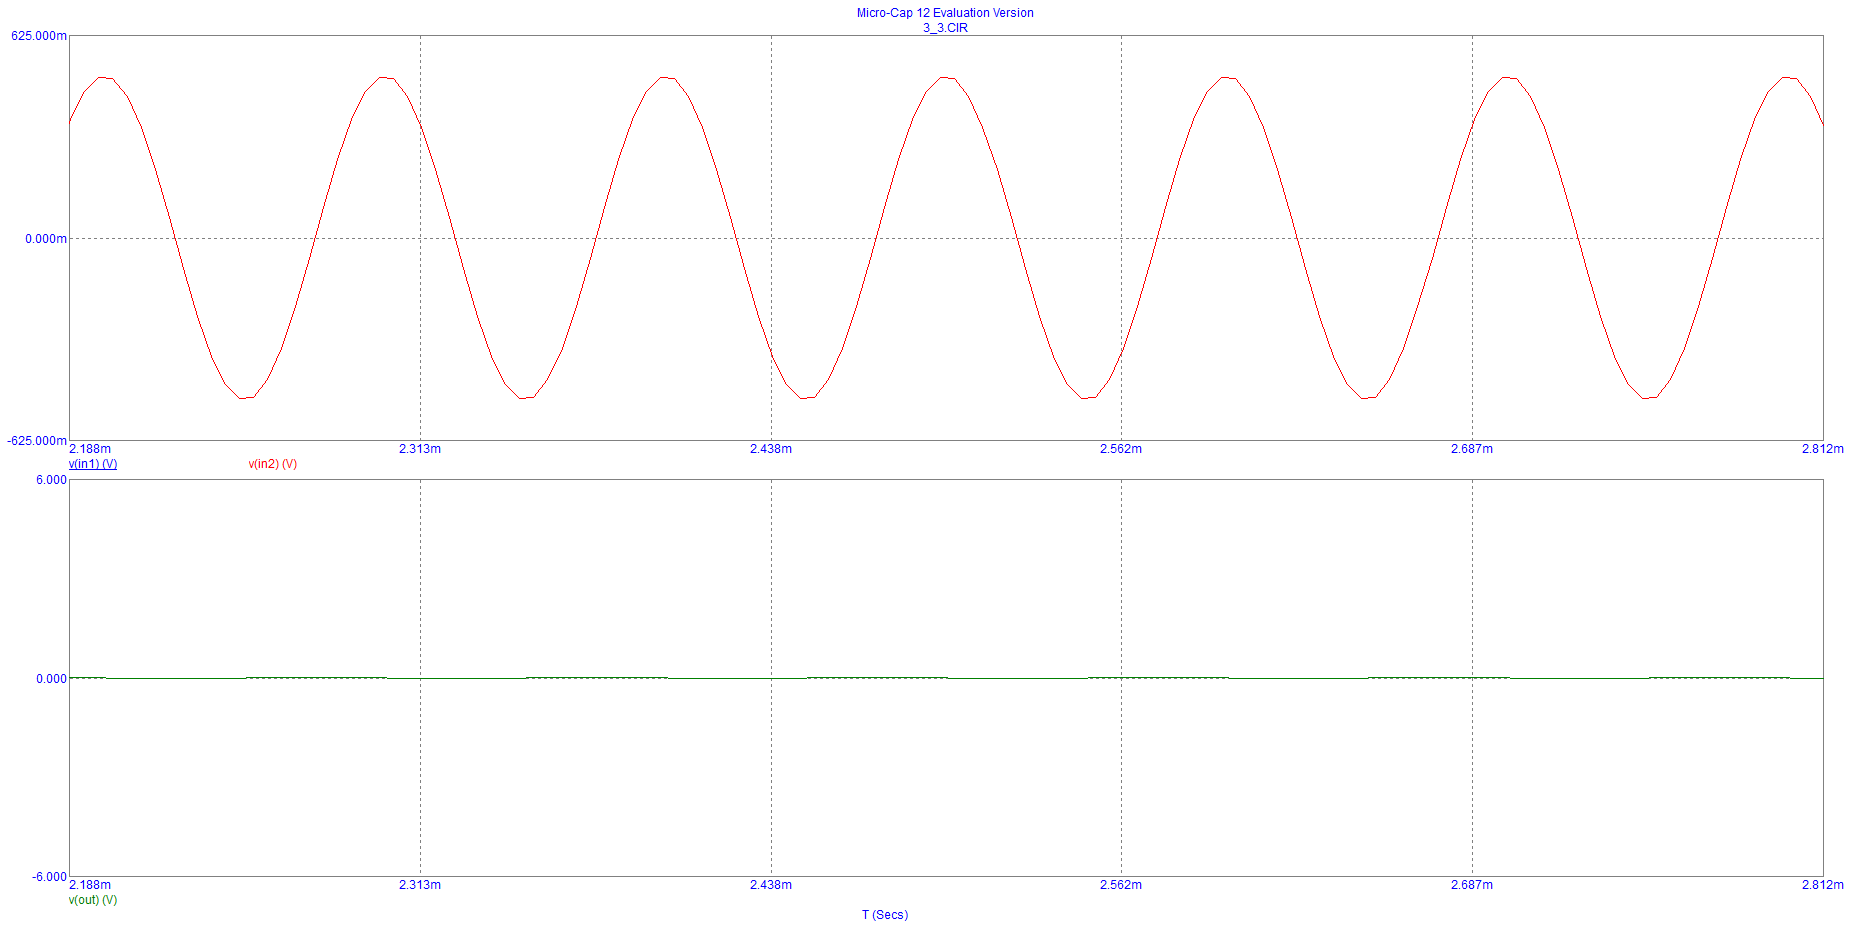
\includegraphics[width=\textwidth]{PC/ukol3/nula_vzstup.png}
    Časový průběh se dvěmy identickými vstupními signály \(U_{pp} = 10\-[V]\) \(f = 1\-[kHz]\)
  \end{minipage}
\end{figure}


% \section*{Průběhy při různých frekvencích}
% \begin{figure}[H]
%   \begin{figure}[H]
%     \begin{minipage}[t]{0.49\textwidth}
%       \(f = 10\-[Hz]\), \(U_{ss-in} = 2.06\-[V]\), \(U_{ss-out} = 22.4\-[V]\)\\
%       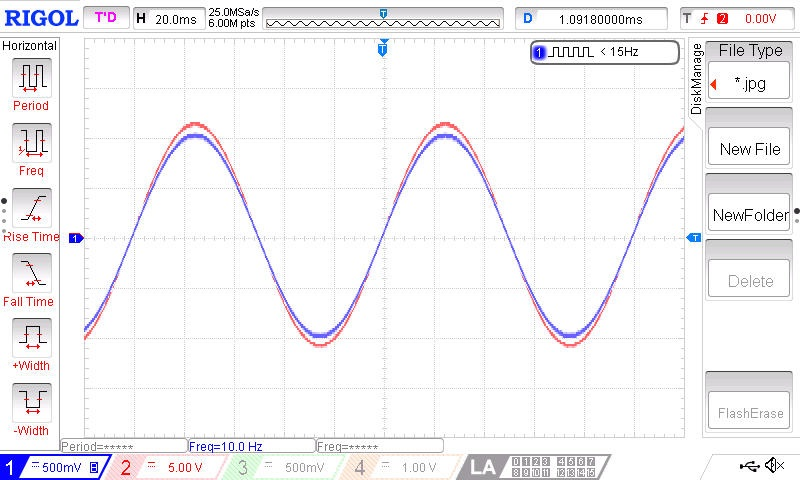
\includegraphics[width=\textwidth]{LAB/NewFile14.jpg}
%     \end{minipage}
%     \hfill
%     \begin{minipage}[t]{0.49\textwidth}
%       \(10\-[kHz]\), \(U_{ss-in} = 2.06\-[V]\), \(U_{ss-out} = 22.6\-[V]\)\\
%       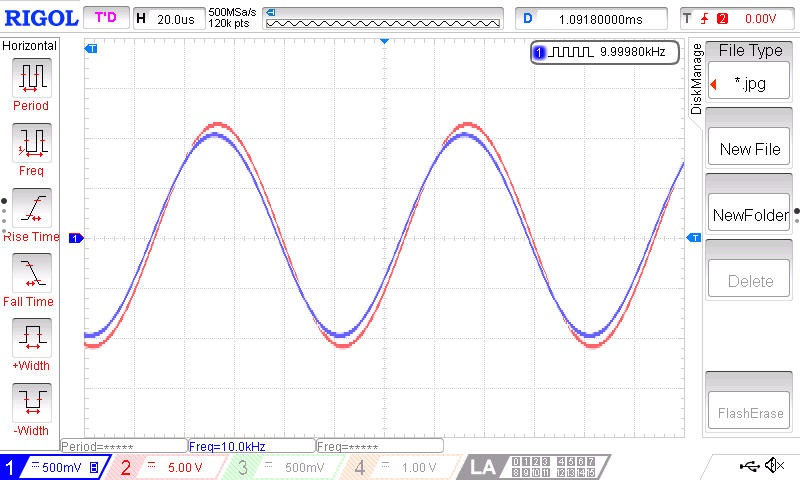
\includegraphics[width=\textwidth]{LAB/NewFile15.jpg}
%     \end{minipage}
%     \vspace{-4mm}
%   \end{figure}
%   \begin{figure}[H]
%     \begin{minipage}[t]{0.49\textwidth}
%       \(100\-[kHz]\), \(U_{ss-in} = 208\-[mV]\), \(U_{ss-out} = 1.82\-[V]\)\\
%       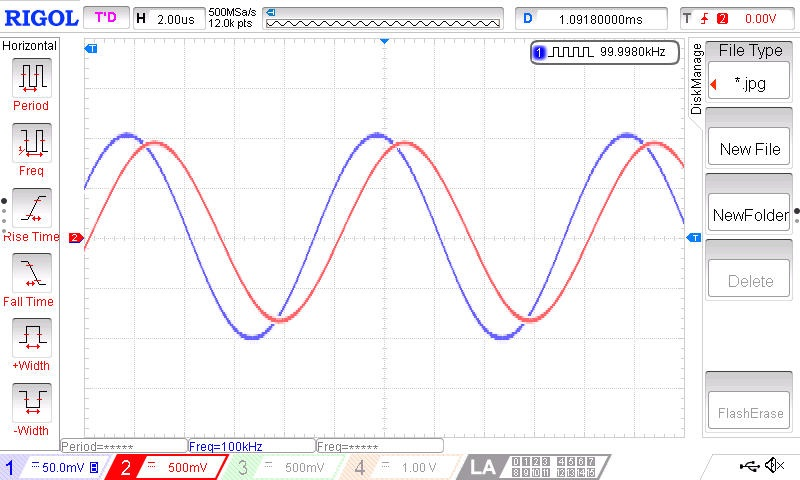
\includegraphics[width=\textwidth]{LAB/NewFile17.jpg}
%     \end{minipage}
%     \hfill
%     \begin{minipage}[t]{0.49\textwidth}
%       \(5\-[MHz]\), \(U_{ss-in} = 208\-[V]\), \(U_{ss-out} = 70\-[mV]\)\\
%       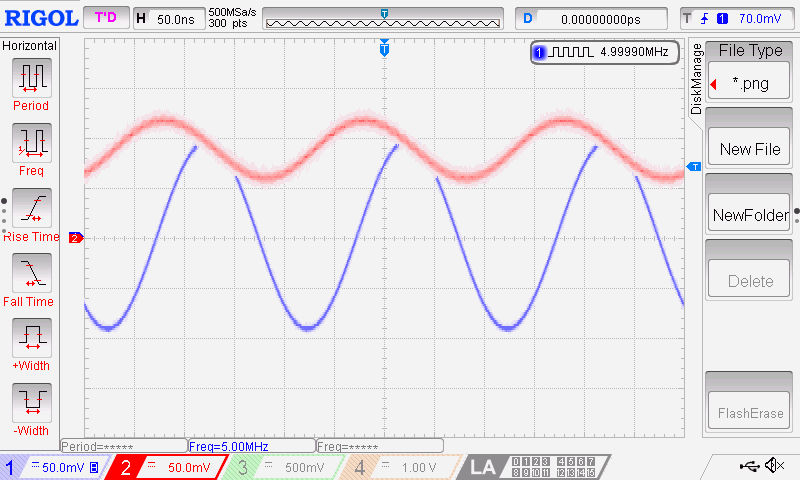
\includegraphics[width=\textwidth]{LAB/NewFile05.png}
%     \end{minipage}
%   \end{figure}
%   \vspace{-2mm}
%   \centering{\obrlabel{sin_prubehy}}
% \end{figure}

% \begin{minipage}[t]{\textwidth}
%   \vspace{-7mm}
%   \begin{tikzpicture}
%     \begin{semilogxaxis}
%       [
%           width=1\textwidth, 
%           height=75mm,
%           title={Amplitudová kmitočtová charakteristika},
%           xlabel={\(f\-[kHz]\)},
%           ylabel={\(A\-[dB]\)},
%           xmin=0.01, xmax=5000,
%           ymin=-10, ymax=23,
%           legend pos=south west,
%       ]
%       \addplot[
%         color=blue,
%         mark=x,
%         ]
%         coordinates {
%           (0.01,  20.72761596 )
%           (10  ,  20.80482438 )
%           (100 ,  18.75704187 )
%           (150 ,  17.19248586 )
%           (200 ,  15.42404781 )
%           (250 ,  13.89628089 )
%           (300 ,  12.64046429 )
%           (350 ,  11.39750616 )
%           (400 ,  10.70226403 )
%           (450 ,   9.679213585)
%           (500 ,   8.519374645)
%           (550 ,   7.252521338)
%           (600 ,   6.503273508)
%           (700 ,   5.242238593)
%           (850 ,   3.766514309)
%           (1000,   2.498774732)
%           (1500,  -0.599264468)
%           (5000,  -9.542425094)
%         };
%       \addlegendentry{\scriptsize \(C_v = 10\-[nF]\)}
%       \addplot[
%         color=red,
%         mark=o,
%         only marks,
%         ]
%         coordinates {
%           (3000,  -3.039151587)
%         };
%       \addlegendentry{\scriptsize Pravděpodobně chybně změřený bod}
%       \addplot[
%         color=black,
%         dotted,
%         thick,
%         mark=o,
%         ]
%         coordinates {
%           (150 ,  17.19248586)
%           (150 ,  -100)
%         };
%       \addplot[
%           dotted,
%           thick,
%           color=black,
%         ]
%         coordinates {
%           (0.01, 0)
%           (5000, 0)
%         };
%         % \addlegendentry{\scriptsize \(C_v = 10\-[nF]\)}
%     \end{semilogxaxis}
%   \end{tikzpicture}
% \end{minipage}

% \begin{figure}[H]
%   \centering
%   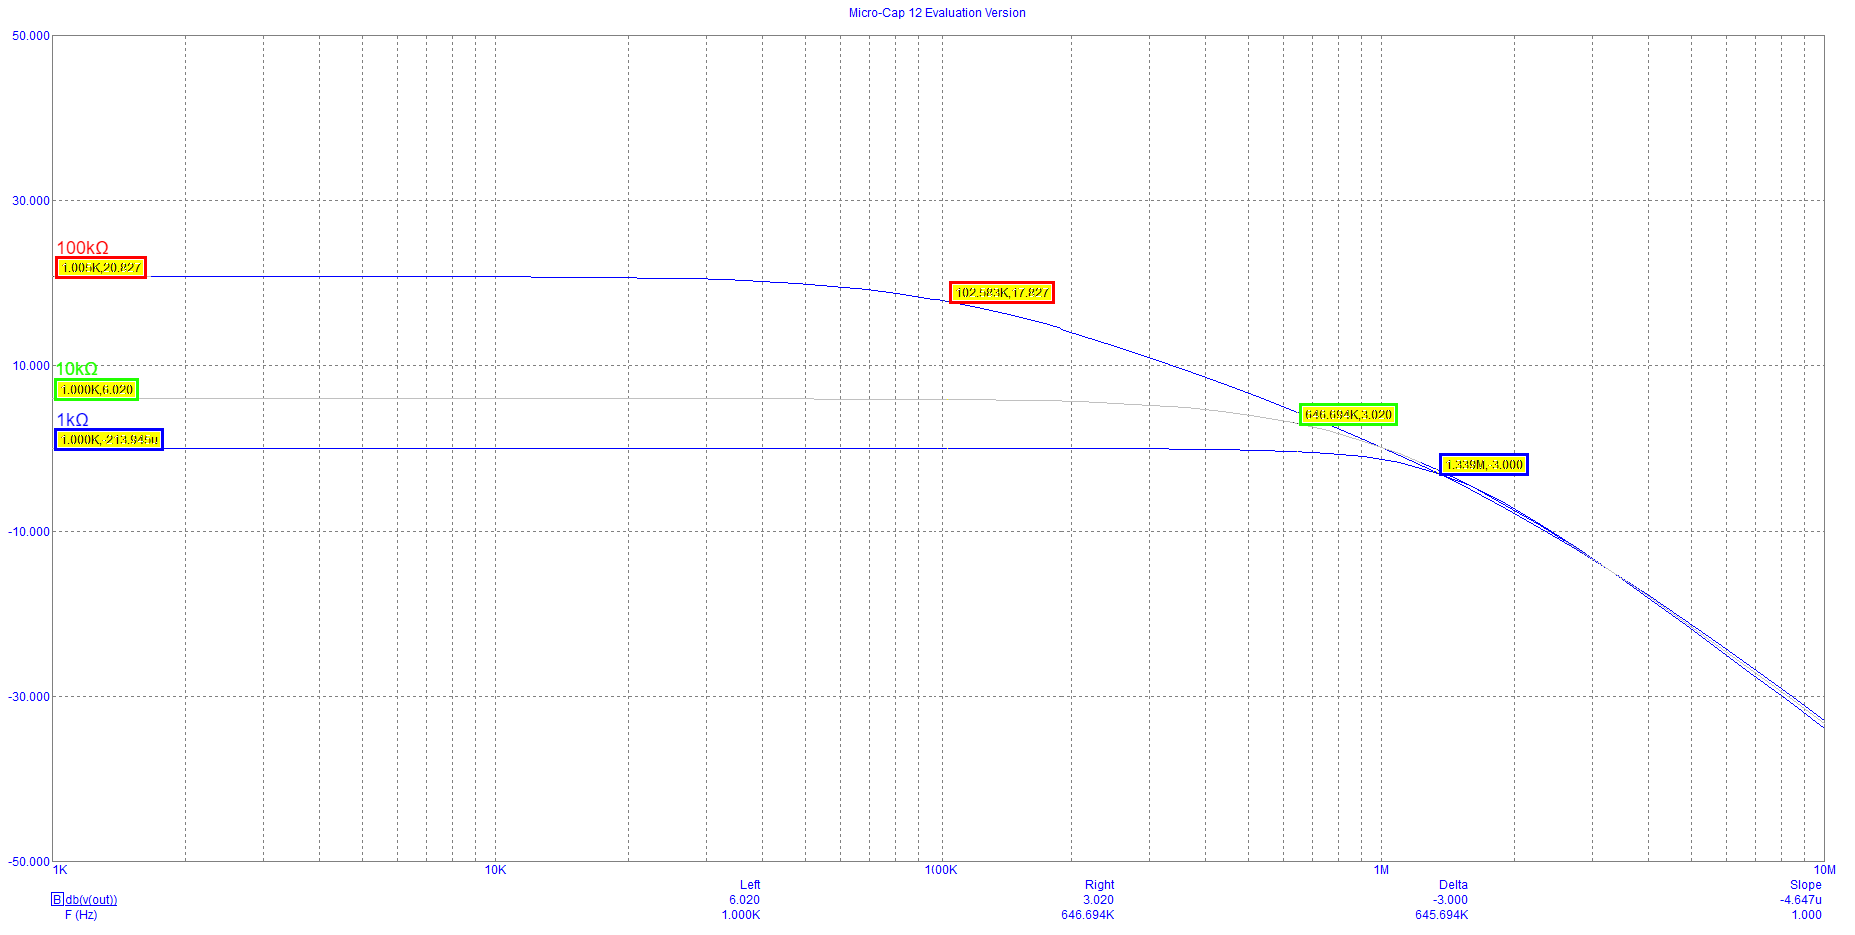
\includegraphics[width=0.8\textwidth]{PC/AC/nein_1k.png}
%   \begin{center}
%     Neinvertující zapojení OZ
%   \end{center}
% \end{figure}

% \begin{figure}[H]
%   \centering
%   \includegraphics[width=0.8\textwidth]{PC/AC/in_1k.png}
%   \begin{center}
%     Invertující zapojení OZ
%   \end{center}
% \end{figure}

% \subsection*{Napětová převodní charakteristika}
% \begin{minipage}[t]{\textwidth}
%   \(R_1 = 1,10,100\-[k\Omega]\)\\
%   \includegraphics[width=\textwidth]{PC/DC/in_1k.png}
% \end{minipage}
% Mimo saturaci se zesílení v napětové převodní charakteristice projeví jako směrnice křivky.

% \begin{figure}[H]
%   \begin{figure}[H]
%     \begin{minipage}[t]{0.49\textwidth}
%       \(R_1 = 1\-[k\Omega]\)\\
%       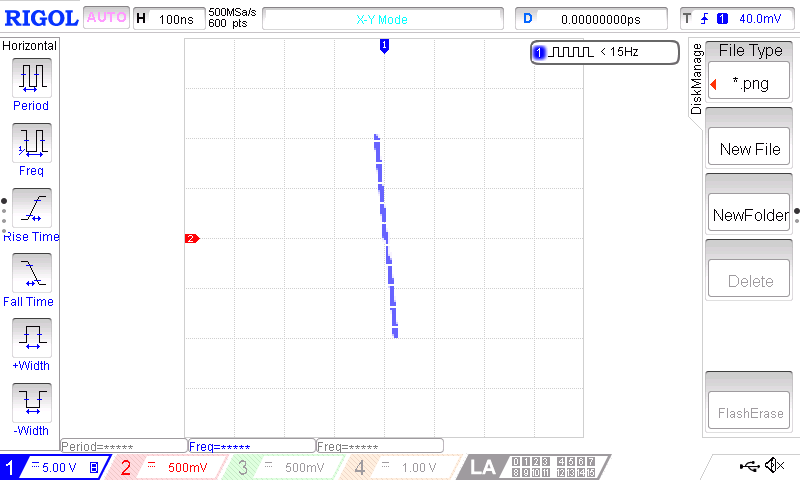
\includegraphics[width=\textwidth]{LAB/NewFile14.png}
%     \end{minipage}
%     \hfill
%     \begin{minipage}[t]{0.49\textwidth}
%       \(R_1 = 10\-[k\Omega]\)\\
%       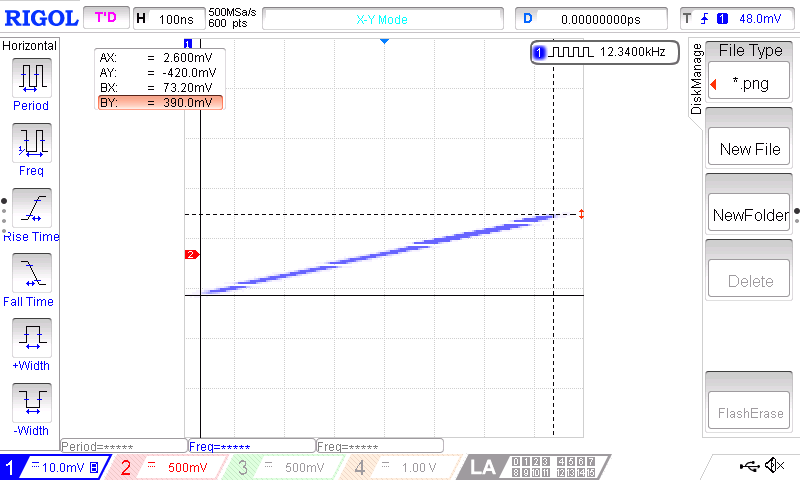
\includegraphics[width=\textwidth]{LAB/NewFile06.png}
%     \end{minipage}
%     \vspace{-4mm}
%   \end{figure}
% \end{figure}

% \begin{figure}[H]
%   \centering
%   \(R_1 = 100\-[k\Omega]\)\\
%   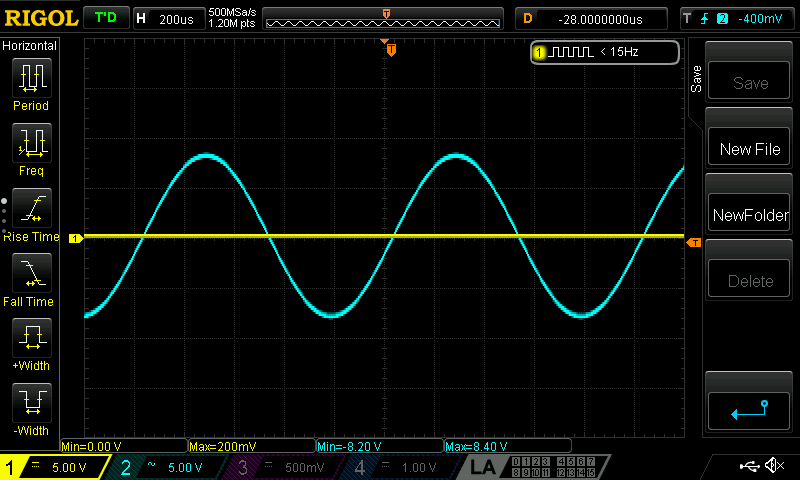
\includegraphics[width=0.5\textwidth]{LAB/NewFile13.png}
% \end{figure}

% \subsection{Závěr}

% \begin{table}[H]
%   % \centering
%   \begin{tabular}{|c|c|c|} 
%     \hline
%     -               & \(SR_{up}\-[V/\mu s]\)  & \(SR_{down}\-[V/\mu s]\) \\ \hline
%     simulace        & 0.5591                  & 0.5533                   \\ \hline
%     měření          & 0.9947                  & 0.8144                   \\\hline
%   \end{tabular}
%   \normalsize
%   \caption{\label{tab_pracovni_bod_rozladeni1}}
% \end{table}

% Při měření mezní rychlosti přeběhu jsme došli ke čtyřem výsledkům (ze simulace a z reálného měření).
% Ze simulace vychází \(RS_{up} = 0.5591\-[V/\mu s], RS_{down} = 0.5533\-[V/\mu s]\).
% Zatím co z reálného měření vyšlo \(RS_{up} = 0.9947\-[V/\mu s], RS_{down} = 0.8144\-[V/\mu s]\).
% Vzhledem k velké odchylce jsem nahlédl do datasheet OZ 1458 \\(www.st.com/resource/en/datasheet/mc1458.pdf strana 6), kde je typická rychlost přeběhu při napájení \(\pm 10\-[V]\) \(SR = 0.8\-[V/\mu s]\), minimální \(0.2\-[V/\mu s]\) a maximální není uvedena.
% Předpokládám proto, že Simulace počítala s modelem, který je podle datasheetu sice možný, ale ne úplně typický.
% % Při měření bylo napájecí napětí \(\pm 15\-[V]\) namísto \(\pm 10\-[V]\) jako v datasheet byla hodnota \(SR\) možná o něco vyšší.

% Reálné průběhy na straně 3.
% Na obrázku \(A\) i \(B\) je zobrazen vstupní a výstupní signál stejného zapojení se stejnou frekvencí \(f = 1\-{kHz}\) ale jinou amplitudou vstupního resp. výstupního signálu. 
% Pokud by nedošlo k saturaci, tak by zesílení \(A\) mělo být u obou průběhů stejně \(A = 13.59\-[V]\).
% Na obrázku \(B\) však dochází k saturaci a signál je tak omezen na napětí v intervalu \(\pm 14.3\-[V]\).

% Při měření frekvenčního rozsahu (strana 4 obr. 1) je vidět, jak se se vzrůstající frekvencí snižuje zesílení a posouvá fáze.
% Navíc je při frekvencích nad 1\-{kHz} vidět, že se k výstupnímu signálu přidává stejnosměrná složka, která je pravděpodobně způsobena asymetrií výstupu zesilovače.
% Na grafu závislosti zesílení na frekvenci je vidět, že první měření, které je oproti maximu sníženo o \(3\-[dB]\), je na frekvenci \(150\-{kHz}\).

% Při simulaci invertujícího zapojení s odporem \(R_1 = 100\-[k\Omega]\) je jasně vidět chyba simulátoru.
% Tato chyba způsobuje, že zapojení, které by mělo mít při nulové frekvenci zesílení \(A = 40\-[dB]\), má zesílení hluboko v záporných číslech.
% Tato chyba je však viditelná i u druhých dvou průběhů, kde se viditelně projevuje na vysokých frekvencích.

% Mimo saturaci se zesílení v napěťové převodní charakteristice zobrazí jako směrnice, v simulaci je to zřetelně viditelné.
% V našem reálném měření je směrnice sice viditelná také, ale je velmi nepřesná.

\end{document}
